% ****** Start of file apssamp.tex ******
%
%   This file is part of the APS files in the REVTeX 4.2 distribution.
%   Version 4.2a of REVTeX, December 2014
%
%   Copyright (c) 2014 The American Physical Society.
%
%   See the REVTeX 4 README file for restrictions and more information.
%
% TeX'ing this file requires that you have AMS-LaTeX 2.0 installed
% as well as the rest of the prerequisites for REVTeX 4.2
%
% See the REVTeX 4 README file
% It also requires running BibTeX. The commands are as follows:
%
%  1)  latex apssamp.tex
%  2)  bibtex apssamp
%  3)  latex apssamp.tex
%  4)  latex apssamp.tex
%
\documentclass[%
 reprint,
%superscriptaddress,
%groupedaddress,
%unsortedaddress,
%runinaddress,
%frontmatterverbose, 
%preprint,
%preprintnumbers,
%nofootinbib,
%nobibnotes,
%bibnotes,
 amsmath,amssymb,
 aps,
%pra,
%prb,
%rmp,
%prstab,
%prstper,
%floatfix,
]{revtex4-2}
\usepackage{kotex}
\usepackage{graphicx}% Include figure files
\usepackage{dcolumn}% Align table columns on decimal point
\usepackage{bm}% bold math
\usepackage{chemformula}
\usepackage{subcaption}

%\usepackage{hyperref}% add hypertext capabilities
%\usepackage[mathlines]{lineno}% Enable numbering of text and display math
%\linenumbers\relax % Commence numbering lines

%\usepackage[showframe,%Uncomment any one of the following lines to test 
%%scale=0.7, marginratio={1:1, 2:3}, ignoreall,% default settings
%%text={7in,10in},centering,
%%margin=1.5in,
%%total={6.5in,8.75in}, top=1.2in, left=0.9in, includefoot,
%%height=10in,a5paper,hmargin={3cm,0.8in},
%]{geometry}

\begin{document}


\title{캐털레이스의 반응속도 예비보고서}

\author{서울대학교 전기정보공학부 2018-12432 박정현}
 \email{alexist@snu.ac.kr}
\date{실험일자: 10/10/2023}% It is always \today, today,
             %  but any date may be explicitly specified

\begin{abstract}
본 실험에서는 감자의 세포에 존재하는 퍼옥시즘의 카탈레이즈가 과산화수소의 분해에서 촉매로 작용하는 점을 이용해 과산화수소 분해 속도를 측정하고 이를 통해 Michaelis–Menten equation와 촉매에 대한 이해도를 높인다.
\end{abstract}

%\keywords{Suggested keywords}%Use showkeys class option if keyword
                              %display desired
\maketitle

%\tableofcontents

\section{\label{sec:level1}Assignment}
\subsection{\label{sec:level2} 1}
아래의 화학반응에서 화학반응 속도는 다음과 같다.
\begin{align}
	\ch{A} &{\overset{k_{1}}{\longrightarrow}} \ch{B}\\
	\frac{d[\ch{B}]}{dt} &= k_{1}[\ch{A}]
\end{align}

아레니우스 식에 의해 $k_{1}$은 식(\ref{eq:arrneiuos})와 같이 나타난다. 여기서 $E_{a}$는 아레니우스 에너지이고 $A$는 $k_{1}$와 같은 차원을 가지는 상수이다. 따라서 온도가 상승함에 따라 $k_{1}$은 증가하게 되고 화학 반응속도는 증가하게 된다. 하지만 온도가 증가함에 따라 단백질은 변성이 일어나게 되면서 단백질의 구조가 바뀌므로 enzyme이 작용하기 위한 key와 lock 관계가 사라지게 되어 activity가 감소하게 된다. [3] 

\begin{align}
	k_{1} &= A\exp\left(-\frac{E_{a}}{RT}\right)\label{eq:arrneiuos}
\end{align}

Protein은 4개의 level을 가지고 있다. Primary structure은 아미노산의 배열, secondary structure은 primary structure의 아미노산들이 서로 상호작용하여 단백질이 나선형, 혹은 평면형으로 배열을 이루는 것이며 각각을 $\alpha-helix$, $\beta-strand$이라고 한다. Tertiary structure는 secondary structure사이의 상호작용으로 3차원 구조를 이룬 단백질 구조이며 Quaternary Structure은 하나 이상의 chain이 존재하는 경우의 단백질이다.[3]
\begin{figure*}[htbp]
	\begin{subfigure}{0.4\textwidth}
		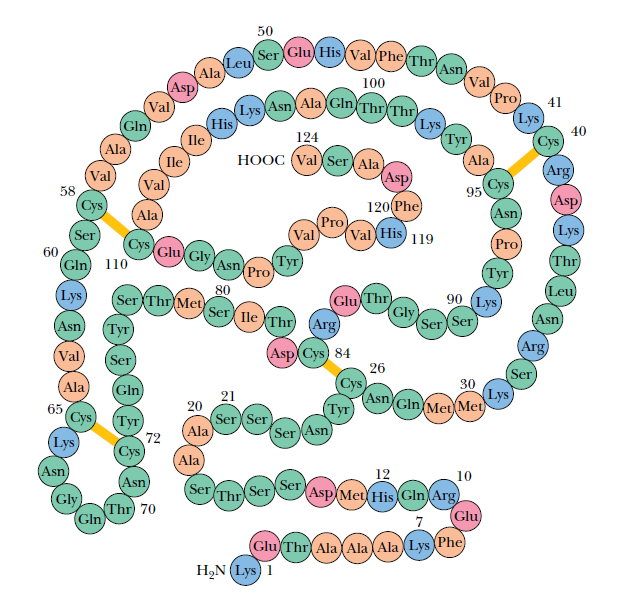
\includegraphics[width = 0.5\linewidth]{First.png}% Here is how to import EPS art
		\caption{\label{fig:First}Primary structure}
	\end{subfigure}
	\begin{subfigure}{0.4\textwidth}
		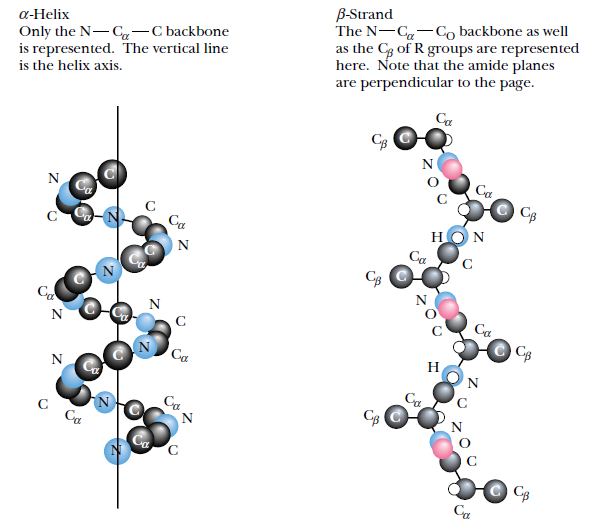
\includegraphics[width = 0.5\linewidth]{Second.png}% Here is how to import EPS art
		\caption{\label{fig:Second}Secondary structure}
	\end{subfigure}

	\begin{subfigure}{0.4\textwidth}
		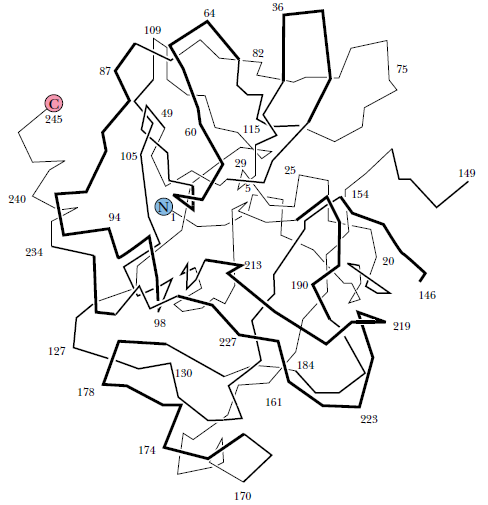
\includegraphics[width = 0.5\linewidth]{Third.png}% Here is how to import EPS art
		\caption{\label{fig:Third}Tertiary structure}
	\end{subfigure}
	\begin{subfigure}{0.4\textwidth}
		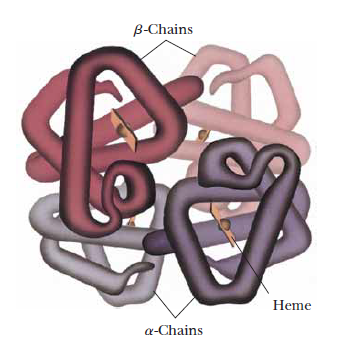
\includegraphics[width = 0.5\linewidth]{Fourth.png}% Here is how to import EPS art
		\caption{\label{fig:Fourth}Quaternary Structure}
	\end{subfigure}
	\caption{\label{fig:Protein}여러 protein구조 }
\end{figure*}

깁스에너지는 $\Delta G = \Delta H - T \Delta S$이다. 아미노산 사이의 이온 결합, 수소결합, 분산력과 같은 결합력은 $\Delta H$를 낮추게 된다. 따라서 저온에서는 작은 $\Delta S$에도 불구하고 아미노산들 사이 가장 많은 상호작용을 하는 tertiary structure,  quaternary structure와 같이 꼬여 있는 상태가 더 안정한 상태이다. 하지만 온도가 증가함에 따라 $\Delta S$에 의한 영향이 증가하게 된다. 이때 꼬여 있는 상태가 아닌 풀어져 있는 protein의 상태가 더 낮은 깁스에너지를 가지게 된다. 따라서 Fig.\ref{fig:denaturation}와 같이 단백질의 구조가 붕괴되는 denaturation가 발생하게 된다.[3]

\begin{figure}[htbp]
	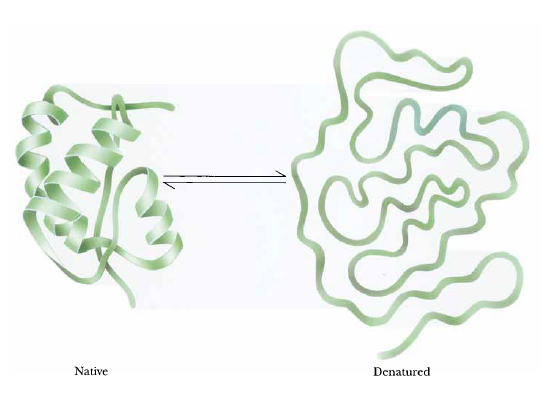
\includegraphics[width = 0.6\linewidth]{denaturation.png}% Here is how to import EPS art
	\caption{\label{fig:denaturation}Denaturation}
\end{figure}

\subsection{\label{sec:level2} 2}
효소와 함께 생성되는 물질의 생성 속도를 나타내는 식(Michaelis–Menten equation)은 식(\ref{eq:mich})와 같다.[2] 단, $[\ch{E}]$는 촉매, $[\ch{S}]$는 반응하는 기질의 농도이다.
\begin{align}
	v &= k_{2}[\ch{ES}] = \frac{k_{2}[\ch{E}]_{0}[\ch{S}]}{[\ch{S}] + K_{m}}\label{eq:mich}
\end{align}

라인웨버-버크 식(Lineweaver-Burk equation)은 식 (\ref{eq:line}) 와 같다.[1] $[\ch{S}]$가 감소함에 따라 반응속도 $v$가 감소함을 알 수 있다. 따라서 $[\ch{S}]$가 최대 값을 가질 때 속도 또한 최대이므로 $[\ch{S}] = \infty$로 두는 경우 최대 속도는 식 (\ref{eq:max})와 같다.

\begin{align}
	\frac{1}{v} &= \frac{1}{k_{2}[\ch{E}]_{0}} + \frac{K_{m}}{k_{2}[\ch{E}]_{0}[\ch{S}]}\label{eq:line}
\end{align}

\begin{align}
	v_{max} &= k_{2}[\ch{E}]_{0} \label{eq:max}\\
	&= 8\times 10^{5}\times 5 \times 10^{-5}M/s\\
	&= 40 [M/s]
\end{align}

최대 속도의 $0.2$배인 경우 식(\ref{eq:mich2})을 만족한다.
\begin{align}
	\begin{split}
		0.2v_{max} &= 0.2 k_{2}[\ch{E}]_{0}\\
		&=\frac{k_{2}[\ch{E}]_{0}[\ch{S}]}{[\ch{S}] + K_{m}}\label{eq:mich2}
	\end{split}
\end{align}

따라서 $[\ch{S}]$는 아래의 식을 만족한다.

\begin{align}
	\frac{[\ch{S}]}{[\ch{S}] + K_{m}} &= 0.2\\
	[\ch{S}] &= \frac{K_{m}}{4}\\
	&= 1\times 10^{-5} [M]
\end{align}

\section{\label{sec:level1}Data \& Result}
\subsection{\label{sec:level2} 1}
시간에 따라 생성된 산소원자의 몰값은 Fig.\ref{fig:v_t}와 같다. 단, 산소원자의 몰값은 이상기체임을 가정하고 $n=\frac{P_{\ch{O2}}V}{RT}$를 이용해 계산하였다. 이때 실험에 사용된 삼각플라스크의 부피는 $100mL$, 그리고 그외의 상수들은 $R=8.3145J/mol K$, $T=300K$으로 두고 계산하였다. 단, 실험 장비에서 측정단위가 $hPa$이므로 $Pa$로 변환하였다.

\begin{figure*}[htbp]
	\begin{subfigure}{0.4\textwidth}
		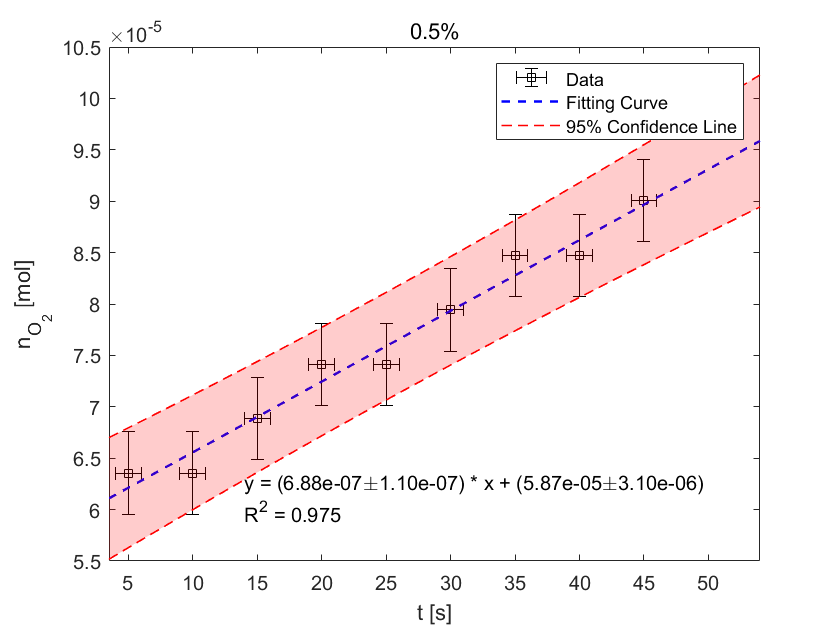
\includegraphics[width = 1\linewidth]{MOL_05.png}% Here is how to import EPS art
		\caption{\label{fig:MOL_05}Denaturation}
	\end{subfigure}
	\begin{subfigure}{0.4\textwidth}
		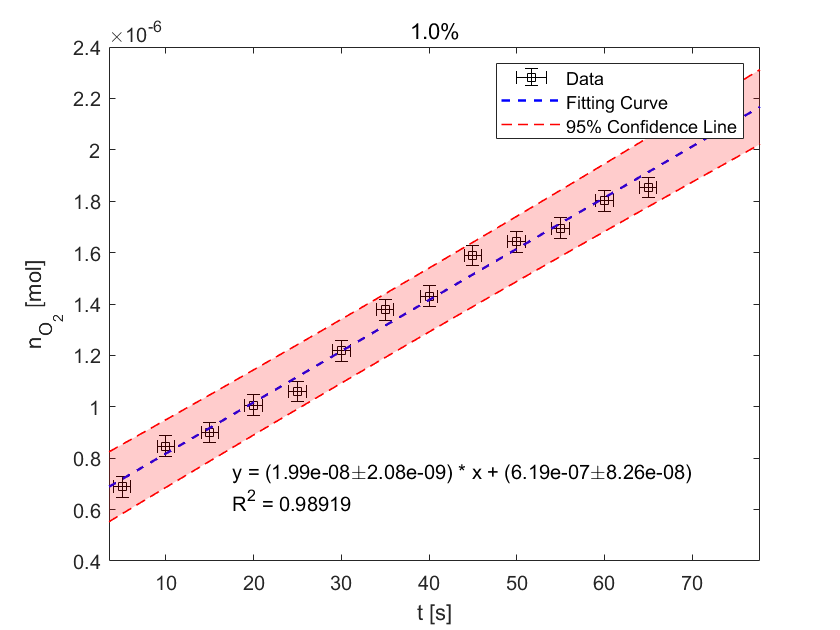
\includegraphics[width = 1\linewidth]{MOL_10.png}% Here is how to import EPS art
		\caption{\label{fig:MOL_10}Denaturation}
	\end{subfigure}

	\begin{subfigure}{0.4\textwidth}
		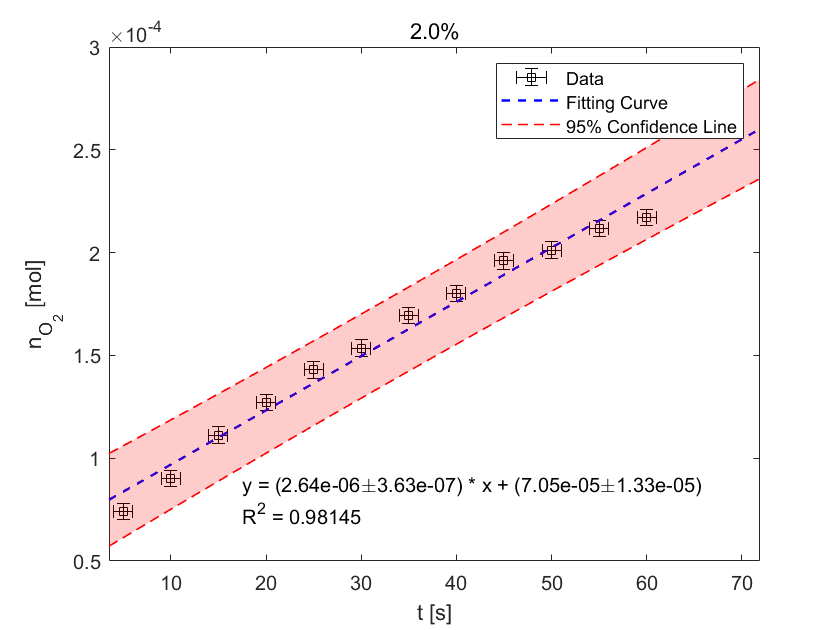
\includegraphics[width = 1\linewidth]{MOL_20.png}% Here is how to import EPS art
		\caption{\label{fig:MOL_20}Denaturation}
	\end{subfigure}
	\begin{subfigure}{0.4\textwidth}
		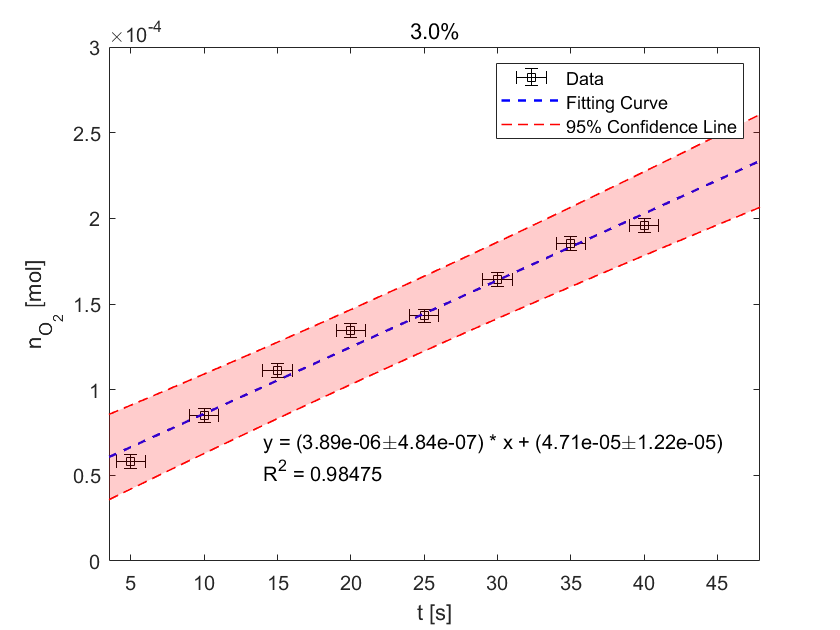
\includegraphics[width = 1\linewidth]{MOL_30.png}% Here is how to import EPS art
		\caption{\label{fig:MOL_30}Denaturation}
	\end{subfigure}

	\begin{subfigure}{0.4\textwidth}
		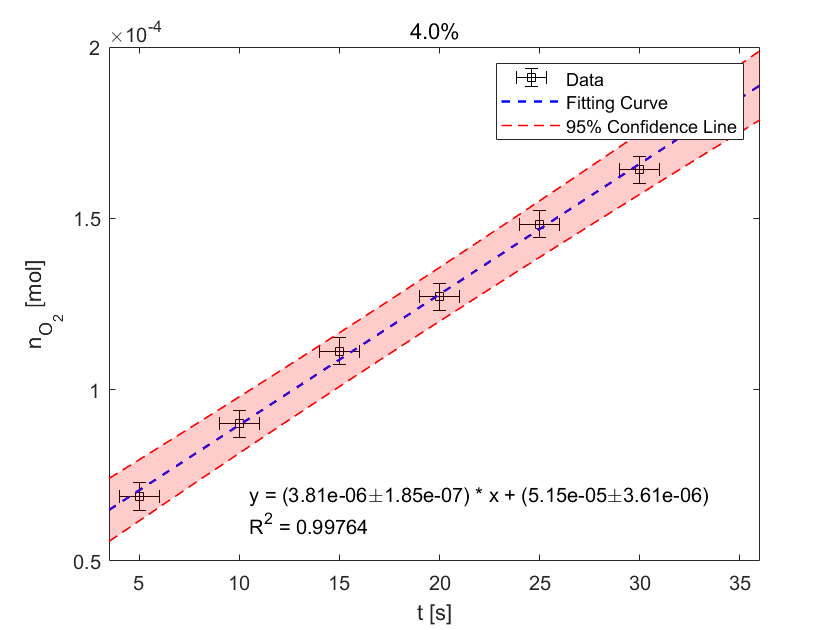
\includegraphics[width = 1\linewidth]{MOL_40.png}% Here is how to import EPS art
		\caption{\label{fig:MOL_40}Denaturation}
	\end{subfigure}
	\begin{subfigure}{0.4\textwidth}
		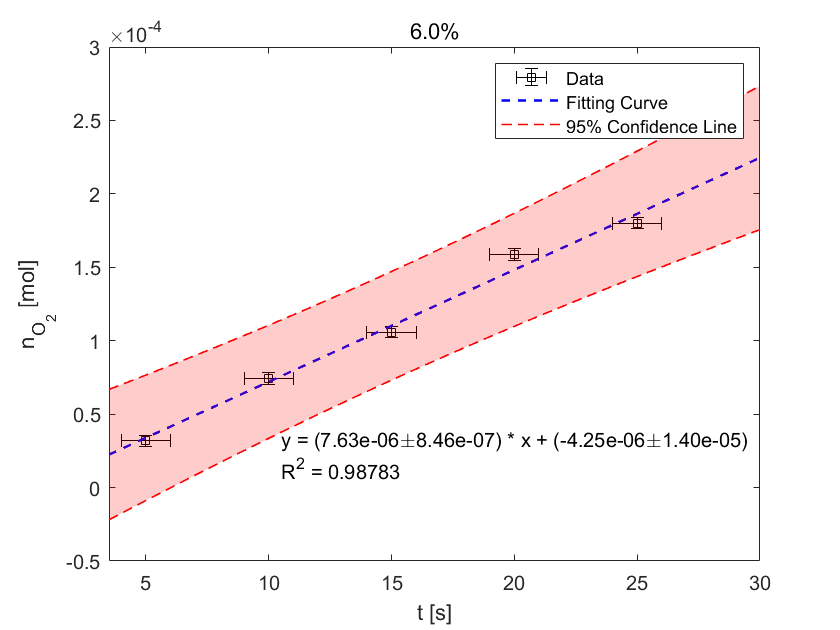
\includegraphics[width = 1\linewidth]{MOL_60.png}% Here is how to import EPS art
		\caption{\label{fig:MOL_60}Denaturation}
	\end{subfigure}
	\caption{\label{fig:v_t}Generate Oxide mole value versus time}
\end{figure*}

기울기를 통해 계산된 속도를 통해 $1/v$, $1/[H_{2}O]$에 대한 그래프는 Fig.\ref{fig:TOT}와 같다. 단, 여기서 $[H_{2}O]$는 반응을 통해 생성된 물의 농도이다. 이 때 화학반응과 생성된 물의 농도는 아래의 관계식을 만족한다.

\begin{align}
	\ch{H2O2} &\rightarrow \ch{H2O + 1/2 O2}\\
	[\ch{H2O}] &= \frac{n_{\ch{O2}}}{2V_{liq}}
\end{align}

\begin{figure}[htbp]
	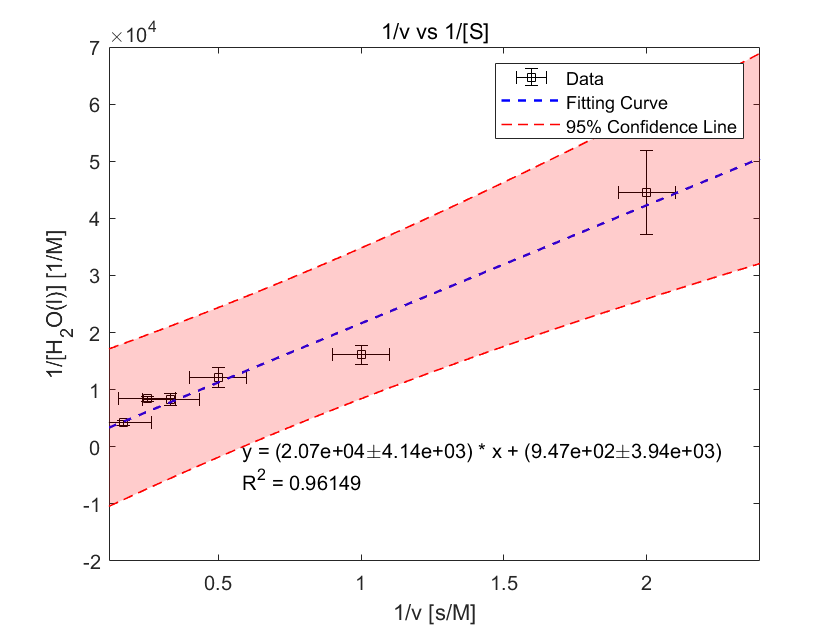
\includegraphics[width = 1.0\linewidth]{TOT.png}% Here is how to import EPS art
	\caption{\label{fig:TOT}Denaturation}
\end{figure}

\section{\label{sec:level1}Conclusion \& Discussion}
$0.5\%$농도에서의 데이터는 큰 오차를 발생시킨다. 따라서 고농도의 데이터만을 이용해 $K_{m}$값을 계산하는 것이 정확한 결과를 도출할 수 있다. 

\section{\label{sec:level1}Reference}
[1] 김. (2010, August 1). 캐털레이스의 반응속도. In \textit{일반화학실험} (1th ed., p. 180).

[2] Oxtoby, D., Gillis, H., \& Campion, A. (2007, April 2). Rates of Chemical and Physical Processes. In \textit{Principles of Modern Chemistry} (6th ed., pp. pp.778-780). Cengage Learning.

[3] Garrett, R. H., \& Grisham, C. M. (2002, January 1). Proteins: Their Biological Functions and Primary Structure. In \textit{Principles of Biochemistry} (pp. 442-443, 115-119, 161). Cengage Learning.

[4]The Catalase-Hydrogen Peroxide System
KINETICS OF CATALATIC ACTION AT HIGH SUBSTRATE CONCENTRATIONS



\end{document}
%
% ****** End of file apssamp.tex ******
